\documentclass[tikz, border=8pt]{standalone}
\usepackage{amsmath}
\usepackage[american]{circuitikz}
\usepackage{iftex}
\ifPDFTeX
\usepackage[scaled=0.92]{helvet}
\renewcommand{\familydefault}{\sfdefault}
\else
\usepackage{fontspec}
\setmainfont{Arial}
\setsansfont{Arial}
\fi
\usetikzlibrary{positioning, shapes, arrows.meta, calc, patterns, decorations.pathmorphing, shadows}

\begin{document}

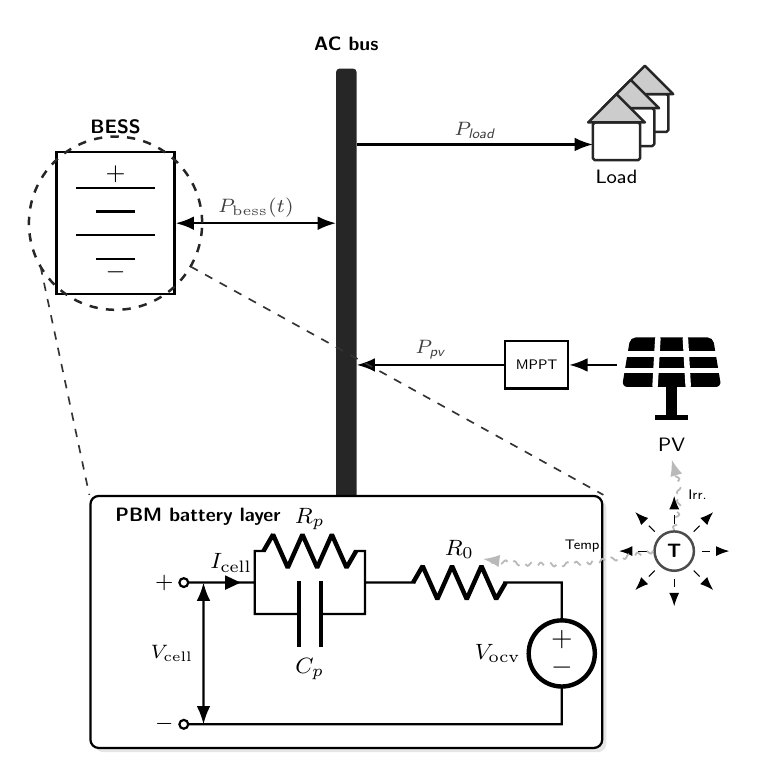
\begin{tikzpicture}[
    font=\sffamily\footnotesize,
    >=Latex,
    thick,
    busbar/.style={draw=black!85, fill=black!85, minimum width=0.15cm, minimum height=5.5cm, rounded corners=1pt},
    sun/.style={circle, draw=black!70, line width=0.9pt, minimum size=0.5cm, fill=white},
    dashed_line/.style={dash pattern=on 3pt off 3pt, draw=black!80, line width=0.6pt},
    power_lab/.style={midway, above, font=\sffamily\scriptsize\itshape, inner sep=1.6pt, fill=white, text=black!75},
    env_arrow/.style={->, dash pattern=on 3pt off 3pt, draw=gray!55, line width=0.65pt, decorate, 
        decoration={snake, amplitude=0.7pt, segment length=3.2pt, post length=2pt}},
    icon/.style={draw=black!85, line width=0.9pt, line join=round, line cap=round},
    iconfillLoad/.style={fill=white}
]

    \tikzset{
        pics/houses3/.style={
            code={
                \begin{scope}[scale=0.8, xshift=0.3cm, yshift=0.3cm]
                    \draw[icon, iconfillLoad, rounded corners=0.7pt] (-0.25,0) rectangle (0.25,0.4);
                    \draw[icon, fill=black!20] (-0.3,0.4) -- (0,0.7) -- (0.3,0.4) -- cycle;
                \end{scope}
                \begin{scope}[scale=0.8, xshift=0.15cm, yshift=0.15cm]
                    \draw[icon, iconfillLoad, rounded corners=0.7pt] (-0.25,0) rectangle (0.25,0.4);
                    \draw[icon, fill=black!20] (-0.3,0.4) -- (0,0.7) -- (0.3,0.4) -- cycle;
                \end{scope}
                \begin{scope}[scale=0.8]
                    \draw[icon, iconfillLoad, rounded corners=0.7pt] (-0.25,0) rectangle (0.25,0.4);
                    \draw[icon, fill=black!20] (-0.3,0.4) -- (0,0.7) -- (0.3,0.4) -- cycle;
                \end{scope}
            }
        },
        pics/solar panel/.style={
            code={
                \fill[black] (-0.3, -1.0) rectangle (0.3, -0.9);
                \fill[black] (-0.1, -0.9) rectangle (0.1, -0.3);
                \fill[black, rounded corners=2pt] (-0.9, -0.4) -- (0.9, -0.4) -- (0.75, 0.5) -- (-0.75, 0.5) -- cycle;
                \begin{scope}
                    \tikzset{gridline/.style={white, line width=2pt, cap=round}}
                    \draw[gridline] (-0.85, -0.1) -- (0.85, -0.1);
                    \draw[gridline] (-0.8, 0.2) -- (0.8, 0.2);
                    \draw[gridline] (-0.3, -0.38) -- (-0.25, 0.48);
                    \draw[gridline] (0.3, -0.38) -- (0.25, 0.48);
                \end{scope}
            }
        }
    }

    \node[busbar] (bus) at (0, 0) {};
    \node[above=0.1cm, font=\sffamily\bfseries\scriptsize] at (bus.north) {AC bus};

    \coordinate (load_pos) at ($(bus.east)+(3.0, 1.8)$);
    \pic[scale=1.5, transform shape] at ($(load_pos)+(0.3, -0.2)$) {houses3};
    \node[below=0.2cm, font=\scriptsize] at ($(load_pos)+(0.3, 0)$) {Load};
    \draw[thick, <-] (load_pos) -- node[power_lab] {$P_{\text{load}}$} (bus.east |- load_pos);

    \coordinate (pv_pos) at ($(bus.east)+(4.0, -1.0)$);
    \pic[scale=0.7, transform shape] at (pv_pos) {solar panel};
    \node[below=0.8cm, font=\scriptsize] at (pv_pos) {PV};
    
    \node[draw, thick, fill=white, minimum width=0.8cm, minimum height=0.6cm, 
          font=\tiny, left=1.3cm of pv_pos] (mppt) {MPPT};
    
    \draw[thick, ->] ($(pv_pos)+(-0.7, 0.0)$) -- (mppt.east);
    \draw[thick, ->] (mppt.west) -- node[power_lab] {$P_{\text{pv}}$} (bus.east |- mppt);

    \coordinate (bess_pos) at ($(bus.west)+(-2.8, 0.8)$);
    \node[draw, thick, fill=white, minimum width=1.5cm, minimum height=1.8cm] (bess_icon) at (bess_pos) {};
    \node[above=0.1cm, font=\sffamily\bfseries\scriptsize] at (bess_icon.north) {BESS};
    \begin{scope}[shift={(bess_pos)}]
        \draw[thick] (-0.5,  0.45) -- (0.5,  0.45);
        \node[font=\small] at (0, 0.62) {$+$};
        \draw[thick] (-0.25, 0.15) -- (0.25, 0.15);
        \draw[thick] (-0.5, -0.15) -- (0.5, -0.15);
        \draw[thick] (-0.25,-0.45) -- (0.25,-0.45);
        \node[font=\small] at (0, -0.62) {$-$};
    \end{scope}
    \draw[thick, <->] (bess_icon.east) -- node[power_lab] {$P_{\mathrm{bess}}(t)$} (bus.west |- bess_icon);

    \coordinate (pbm_anchor) at ($(bus.south)+(0, -1.5)$);
    \node[draw, thick, rounded corners=3pt, fill=white, minimum width=6.5cm, minimum height=3.2cm, 
          drop shadow={shadow xshift=1.5pt, shadow yshift=-1.5pt, opacity=0.2}] (pbm_box) at (pbm_anchor) {};
    \node[anchor=west, font=\sffamily\bfseries\scriptsize] at ($(pbm_box.north west)+(0.2,-0.28)$) {PBM battery layer};

    \draw[dashed, black!85, line width=0.9pt] (bess_pos) circle (1.1cm);
    \draw[dashed_line] ($(bess_pos)+(210:1.1cm)$) -- (pbm_box.north west);
    \draw[dashed_line] ($(bess_pos)+(330:1.1cm)$) -- (pbm_box.north east);

    \coordinate (ckt_base) at ($(pbm_box.west)+(1.2, -0.4)$);
    \begin{scope}[shift={(ckt_base)}]
        \draw (0, 0.9) node[left] {$+$} coordinate (pos_term)
            to[short, o-] ++(0.3, 0)
            to[short, i=$I_{\mathrm{cell}}$] ++(0.6, 0) coordinate (pre_RC)
            -- ++(0, 0.4) to[R, l=$R_p$] ++(1.4, 0) -- ++(0, -0.4) coordinate (post_RC)
            (pre_RC) -- ++(0, -0.4) to[C, l_=$C_p$] ++(1.4, 0) -- (post_RC)
            to[short] ++(0.3, 0) coordinate (pre_R)
            to[R, l=$R_{0}$] ++(1.8, 0) coordinate (post_R)
            to[short] ++(0.4, 0)
            to[V, l_=$V_{\mathrm{ocv}}$] ++(0, -1.8)
            to[short, -o] ++(-4.8, 0) coordinate (neg_term) node[left] {$-$};
        
        \coordinate (Rint_center) at ($(pre_R)!0.5!(post_R) + (0,0.1)$);
        \draw[<->] ($(pos_term)+(0.25,0)$) -- node[left, font=\scriptsize] {$V_{\mathrm{cell}}$} ($(neg_term)+(0.25,0)$);
    \end{scope}

    \coordinate (sun_pos) at ($(pbm_box.east)+(0.9, 0.9)$);
    \node[sun] (sun) at (sun_pos) {};
    \foreach \angle in {0, 45, ..., 315} {
        \draw[->, dashed, thin] ($(sun_pos) + (\angle:0.35cm)$) -- ($(sun_pos) + (\angle:0.7cm)$);
    }
    \node[font=\sffamily\scriptsize\bfseries] at (sun_pos) {T};

    \coordinate (pv_target) at ($(pv_pos)+(0.0, -1.2)$);
    \draw[env_arrow] (sun.north) to[bend right=15] 
        node[midway, right, font=\tiny, align=left] {Irr.} (pv_target);

    \coordinate (temp_target) at ($(Rint_center)+(0.3, 0.2)$);
    \draw[env_arrow] (sun.west) to[bend left=10] 
        node[pos=0.4, above, font=\tiny, align=center] {Temp.} (temp_target);

\end{tikzpicture}

\end{document}
